\chapter[Topic: General Cash Flows and Portfolios]{Topic: General Cash Flows and Portfolios (15\%-20\%)}

\subsection{Information}

\begin{distributions}[Objective]
The Candidate will understand key concepts concerning yield curves, rates of return, and measures of duration and convexity, and how to perform related calculations.
\end{distributions}

\begin{outcomes}[Learning outcomes]
The candidate will be able to:
\begin{enumerate}[label = \alph*), leftmargin = *]
	\item	Define and recognize the \textit{definitions} of the following terms:
		\begin{itemize}[leftmargin = *]
		\item	Yield rate / rate of return;
		\item	Dollar-weighted rate of return;
		\item	Time-weighted rate of return;
		\item	Current value;
		\item	Duration	 (Macaulay and modified);
		\item	Convexity (Macaulay and modified);
		\item	Portfolio;
		\item	Spot rate;
		\item	Forward rate;
		\item	Yield Curve;
		\item	Stock price;
		\item	Stock dividend.
		\end{itemize}
	\item	Calculate:
		\begin{itemize}[leftmargin = *]
		\item	The dollar-weighted and time-weighted rate of return;
		\item 	The duration and convexity of a set of cash flows;
		\item	Either Macaulay or modified duration given the other;
		\item	The approximate change in present value due to a change in interest rate using a 1st-order:
			\begin{itemize}[leftmargin = *]
			\item	Linear approximation based on modified duration;
			\item	Approximation based on Macaulay duration.
			\end{itemize}
		\item	The price of a stock using the dividend discount model;
		\item	The present value of a set of cash flows, using a yield curve developed from forward and spot rates.
		\end{itemize}
\end{enumerate}
\end{outcomes}

\begin{ASM_chapter}[Related lessons ASM]
Section 5: 
\begin{itemize}[leftmargin = *]
	\item	\nameref{L.-5a}
	\item	\nameref{L.-5b}
	\item	\nameref{L.-5c}
	\item	\nameref{L.-5d}
	\item	\nameref{L.-5e}
	\item	\nameref{L.-5f}
\end{itemize}
Section 8: 
\begin{itemize}[leftmargin = *]
	\item	\nameref{L.-8a}
	\item	\nameref{L.-8b}
	\item	\nameref{L.-8c}
\end{itemize}
Section 10: 
\begin{itemize}[leftmargin = *]
	\item	\nameref{L.-10a}
	\item	\nameref{L.-10b}
	\item	\nameref{L.-10c}
	\item	\nameref{L.-10d}
	\item	\nameref{L.-10e}
	\item	\nameref{L.-10f}
	\item	\nameref{L.-10g}
\end{itemize}
Section 11: 
\begin{itemize}[leftmargin = *]
	\item	\nameref{L.-11a}
\end{itemize}
\end{ASM_chapter}

\subsection{Chapter summaries}

\begin{CHPT_SUMM_AUTO}[label = {L.-5a}]{5a. Net Present Value and Internal Rate of Return}
\paragraph{Net Present Value (NPV)}
Method consists of comparing the NPV of the cash inflows and outflows.
\begin{description}
	\item[$A_{t}$]	Cash inflow at time $t$ ("\textbf{A}ssets").
	\item[$L_{t}$]	Cash outflow at time $t$ ("\textbf{L}iabilities").
	\item[$i$]	The rate we believe could be earned on alternative investments with the \hl{same degree of risk}.
		\begin{itemize}[leftmargin = *]
		\item	a.k.a. the \textbf{cost of capital}, opportunity cost of capital or the interest preference rate.
		\end{itemize}
	\item[$P(i)$]	NPV at rate $i$.
		\begin{itemize}[leftmargin = *]
		\item	This notation is used as the NPV is a function of the interest rate $i$.
		\end{itemize}
\end{description}
\begin{align*}
	P(i)
	&=	\sum A_{t} v^{t} - \sum L_{t} v^{t}
	=	\sum (A_{t} - L_{t}) v^{t}
\end{align*}

\tcbline

\paragraph{Yield Rate or Internal Rate of Return (IRR)}
Because $P(i)$ can be negative or positive depending on the interest rate, we deduce there must be a rate such that it is equal to $0$. In fact, the solution such that $P(i) = 0$ is the IRR:
\begin{align*}
	P(i)
	&=	\sum (A_{t} - L_{t}) v^{t}
	=	0
\end{align*}

\tcbline

\paragraph{Note}	This can be solved by the calculator.
\begin{itemize}[leftmargin = *]
	\item	Access the cashflows worksheet through \colorbox{arsenic}{\textcolor{white}{CF}}.
	\item	Cash flows are the \texttt{C01} options.
	\item	The \texttt{F01} options are the frequency for the payments.
	\item	Press the \colorbox{arsenic}{\textcolor{white}{NPV}} button after cashflows are entered, enter the interest rate, then go down to the \texttt{NPV} field and hit \colorbox{arsenic}{\textcolor{white}{CPT}}.
	\item	To obtain the IRR of a series of cashflows, press the \colorbox{arsenic}{\textcolor{white}{IRR}} button followed by \colorbox{arsenic}{\textcolor{white}{CPT}} after entering the series.
\end{itemize}
\end{CHPT_SUMM_AUTO}

\begin{CHPT_SUMM_AUTO}[label = {L.-5b}]{5b. Is the Yield Rate Unique?}
For most transactions there is one positive solutions however in the theory there are as many as the degree of the polynomial in the equation $P(i)$ (i.e. the largest exponent). Situations where it is not unique are often somewhat artificial but they can happen. \\

This sections highlights the limitations of the yield rate as an answer to \og Is this a good investment? \fg{} and that there are other methods which are not part of the syllabus to answer it.
\end{CHPT_SUMM_AUTO}

\begin{CHPT_SUMM_AUTO}[label = {L.-5c}]{5c. Reinvestment Rates}
Two general scenarios:
\begin{enumerate}[leftmargin = *]
	\item	Suppose we have $1$ in a fund crediting interest at rate $i$.\\
			Annually, we withdraw the interest and reinvest it into another fund earning $i'$.
			Their accumulated value at the end of $n$ years is :
			\begin{align*}
			AV
			&=	1 + i \sx{\angln i'}
			\end{align*}
	\item	Suppose that we deposit $1$ in a fund crediting interest at rate $i$ at the beginning of each year.\\
			Annually, we withdraw the interest and reinvest it into another fund earning $i'$.
			Their accumulated value at the end of $n$ years is :
			\begin{align*}
			AV
			&=	n + i \Is{\angln i'}
			\end{align*}
\end{enumerate}
\end{CHPT_SUMM_AUTO}

\begin{CHPT_SUMM_AUTO}[label = {L.-5d}]{5d. Yield Rate Earned by a Fund}
\begin{description}
	\item[$A$]	Amount in the fund at the beginning of the year.
	\item[$B$]	Amount in the fund at the end of the year.
	\item[$C_{t}$]	Deposit in or withdrawal from (positive or negative) the fund at time $t$.
	\item[$C$]	Net sum of the deposits / withdrawals.
		\begin{align*}
		C	&=	\sum C_{t}
		\end{align*}
	\item[$I$]	Amount of interest earned in the period.
		\begin{align*}
		I	&=	B - A - C
		\end{align*}
\end{description}
%We thus have the relation $B = A(1 + i) + \sum C_{t} (1 + i)^{1 - t}$ which can be approximated with simple interest $B \approx A(1 + i) + \sum C_{t} [1 + (1 - t)i]$. We use this to isolate $i$ with $C = \sum C_{t}$ representing the net sum of the deposits / withdrawals:
%\begin{align*}
%	i
%	&\approx	\frac{B - A - C}{A + \sum C_{t} (1 - t)}
%\end{align*}

%We then define:
%and rewrite the approximation with the assumption that the net amount of deposits / withdrawals occurs at time $1/2$:
With this we approximate the yield rate as:
\begin{align*}
	i
	\approx	\frac{2I}{A + B - I}
\end{align*}
\end{CHPT_SUMM_AUTO}

\begin{CHPT_SUMM_AUTO}[label = {L.-5e}]{5e. Dollar-Weighted and Time-Weighted Interest Rates}
\textbf{Dollar-weighted} consists of isolating $i$ from the cashflows with the assumption of simple interest.
\textbf{Time-weighted} ignores how much time each transaction spent accumulating and multiplies balances. It is easy to make a mistake and best practice to draw a table. \\

See Coaching Actuaries' formula sheet for a good visualisation.
\end{CHPT_SUMM_AUTO}

\begin{CHPT_SUMM_AUTO}[label = {L.-5f}]{5f. Portfolio Methods and Investment Year Methods}
\begin{description}
	\item[Portfolio Method]	The yield rate is proportional to the amount members invested regardless of the date they invested.
		\begin{itemize}[leftmargin = *]
		\item	May seem unfair, but if there are losses the new members are the losers.
		\item	This is how savings accounts, TFSAs, etc. operate.
		\end{itemize}
	\item[Investment Year Method (IYM)]	The yield rate is proportional to the date members invested.
		\begin{itemize}[leftmargin = *]
		\item	There are several methods, but this is \hl{no longer on the syllabus}.
		\item	This is how a Certificate of Deposit (CD) operates.
		\end{itemize}
\end{description}
\end{CHPT_SUMM_AUTO}

\begin{center}
\begin{tikzpicture}
\clip node (m) [
	matrix,
	matrix of nodes,
	fill = black!20, % alternating rows color
	inner sep = 1pt, % width of exterior line
	nodes in empty cells,
	nodes = {
		minimum height = 3cm,
		minimum width = 3cm,
		anchor = center,
		outer sep = 0,
		font = \sffamily
	},
	row 1/.style = {
		nodes = {
			fill = ballblue,  % header colour
			text = white,
			font = \bfseries
		}
	},
	column 1/.style = {
		text width = 4cm, 
		align = center,
		nodes = {
			font = \bfseries
		},
		every even row/.style = {
			nodes = {
				fill = white
			}
		}
	},
	column 2/.style = {
		text width = 3.5cm,
		align = center,
		every even row/.style = {nodes = {fill = white}},
	},
	column 3/.style = {
		text width = 3.5cm,
		align = center,
		every even row/.style = {nodes = {fill = white}},
	},
	column 4/.style = {
		text width = 3.5cm,
		align = center,
		every even row/.style = {nodes = {fill = white}},
	},
%	row 1 column 1/.style = {nodes = {fill = gray}},
	prefix after command = {
		[rounded corners = 4mm] (m.north east) rectangle (m.south west)
	}
] {
	Feature	&	Bond	&	Preferred Stock	&	Common Stock	\\
	Nature of the Security	&	Loan to a company or governmental unit.	&	Capital investment in a corporation, with no guarantee of a return.	&	Same as preferred stock.	\\
	Relation of the Investor to the Company	&	\textbf{Creditor} of (or lender to) the company.	&	\textbf{Part-owner} of the company, with the right to vote for the Board of Directors and on other corporate matters.	&	Same as preferred stock.	\\
	Term of the Investment	&	Usually fixed at issue although some may be called before.	&	Generally has no maturity date.	&	Same as preferred stock.	\\
	Investment Returns	&	Periodic coupons throughout the term plus the face amount on maturity.	&	Fixed periodic dividends.	&	Periodic dividends at the company's discretion.	\\
	Price	&	Varies with current interest rates. Default risk may also affect the price.	&	Varies with current interest rates as the dividends are a fixed amount.	&	Very volatile.	\\
	Degree of Security	&	First in degree of security as payments on debt are made before issuing dividends.	&	Preferred stock dividends are paid before common stock dividends can be.	&	Last in degree of security.	\\
};
\end{tikzpicture}
\end{center}

\begin{CHPT_SUMM_AUTO}[label = {L.-8a}]{8a. Bonds Preferred Stock and Common Stock}
A company can raise money with:
\begin{description}
	\item[Debt]	Bonds are a form of debt.
	\item[Equity]	Stocks are a form of equity.
\end{description}

\

There are a few types of bonds:
\begin{description}
	\item[Junk bonds]	Often used as a way to finance the takeover of a one corporation by another and are much riskier than investment grade bonds.
	\item[Investment grade bonds]	Bonds with a very low risk of default.
	\item[Zero-coupon bonds]	Bond without coupons in which the investor receives a single lump sum payment at maturity.
\end{description}
\end{CHPT_SUMM_AUTO}

\begin{CHPT_SUMM_AUTO}[label = {L.-8b}]{8b. Price of a Share of Stock}
The price of a typical preferred stock (or perpetual bond) is the PV of a perpetuity of the dividends (or coupons):
\begin{align*}
	P	&=	\frac{Fr}{i}
\end{align*}

%%%	--------------------
%%%	NOTE:
%%%	+	Don't think I wrote this right, need to verify for common vs preferred stock.
%%%	--------------------
With the \textbf{dividend discount model}, or \textbf{the discounted cash flow technique}, if the dividends $D$ for a common stock increase by a constant ratio of $(1 + k)$ we obtain:
\begin{align*}
	P	&=	\frac{D}{i - k}
\end{align*}
However this method is \textit{theoretical} as the future dividends of common stock are difficult to predict.
\end{CHPT_SUMM_AUTO}

\begin{CHPT_SUMM_AUTO}[label = {L.-8c}]{8c. Other Financial Instruments}
\begin{description}
	\item[Sector funds]	Mutual funds with investments in a particular sector.
	\item[Index funds]	No active management of the fund, it reproduces the results of the index it follows.
	\item[Load]	Commission to buy shares, but there are many \textbf{no-load} mutual funds as well.
	\item[Money Market Mutual Funds]	Invest in very safe, short-term debt instruments (for example, T-bills).
		\begin{itemize}[leftmargin = *]
%		\item	Usually no government deposit insurance.
		\item	Interest rates frequently change.
		\end{itemize}
	\item[Certificate of Deposit]	Deposit in a bank for a fixed term with a guaranteed interest rate.
		\begin{itemize}[leftmargin = *]
		\item	There is usually an interest penalty for an early withdrawal.
%		\item	Deposit insurance.
		\item	Interest rates frequently change.
		\end{itemize}
\end{description}
\end{CHPT_SUMM_AUTO}

\begin{CHPT_SUMM_AUTO}[label = {L.-10a}]{10a. Duration of a Single Cash Flow}
\begin{description}
	\item[Fixed-income investments]	Investments that pay \textbf{fixed} (\textit{known}) amounts of future income.
		\begin{itemize}[leftmargin = *]
		\item	e.g., bond coupons, mortgage payments, etc.
		\item	Opposite of investments with \textbf{unknown} future amounts.\\
				e.g., dividends.
		\end{itemize}
\end{description}
\begin{itemize}[leftmargin = *]
	\item	Given that the \textit{future} income is fixed, the \textit{present} value of the investments depends on \textit{current} interest rates.\\
			Thereby, companies need tools to measure the impact that changes in interest rates have on asset values.\\
			e.g., duration, convexity, etc.
	\item	An issue arising from this is that a financial institution \textbf{guarantees} \textit{future} payments.\\
			However, its ability to fulfill them depends on the value of the investment it holds.
\end{itemize}
\begin{description}
	\item[Immunization]	Protection against the effect of future changes in interest rates.
		\begin{itemize}[leftmargin = *]
		\item	The institution tries to "immunize" itself from the impact of changes in interest rates.
		\end{itemize}
\end{description}

	\tcbline

\begin{description}
	\item[Price sensitivity]	of a bond to a change in the interest rate.
		\begin{itemize}[leftmargin = *]
		\item	i.e., the percentage change in price.
		\item	The greater the term of the bond, the more sensitive its price.
		\end{itemize}
	\item[Duration]	The time remaining to a single cash inflow or outflow.
\end{description}

Given the shape of the price/yield curve, a decrease in the interest rate will lead to a larger difference in price than an increase.
\begin{center}
	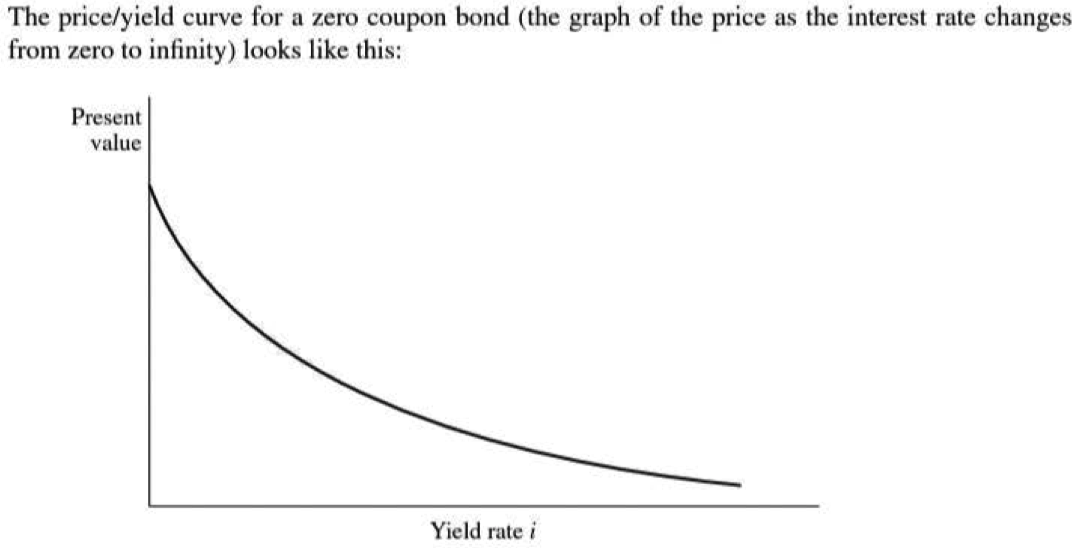
\includegraphics[scale=0.3]{img/duration-SCF.png}
\end{center}
\end{CHPT_SUMM_AUTO}

\begin{CHPT_SUMM_AUTO}[label = {L.-10b}]{10b. Macaulay Duration}

\end{CHPT_SUMM_AUTO}

\begin{CHPT_SUMM_AUTO}[label = {L.-10c}]{10c. Macaulay Duration as a Measure of Price Sensitivity}

\end{CHPT_SUMM_AUTO}

\begin{CHPT_SUMM_AUTO}[label = {L.-10d}]{10d. Modified Duration}

\end{CHPT_SUMM_AUTO}

\begin{CHPT_SUMM_AUTO}[label = {L.-10e}]{10e. Duration of a Portfolio}

\end{CHPT_SUMM_AUTO}

\begin{CHPT_SUMM_AUTO}[label = {L.-10f}]{10f. Change in Duration As Time Goes By}

\end{CHPT_SUMM_AUTO}

\begin{CHPT_SUMM_AUTO}[label = {L.-10g}]{10g. Convexity}

\end{CHPT_SUMM_AUTO}

\begin{CHPT_SUMM_AUTO}[label = {L.-11a}]{11a. Spot Rates and Forward Rates}

\end{CHPT_SUMM_AUTO}

